\documentclass[11pt, a4paper]{article}


% Modules essentiels
\usepackage[french]{babel}
\usepackage[T1]{fontenc}
\usepackage[hmargin=2.5cm, vmargin=2.5cm]{geometry}
\usepackage[utf8]{inputenc}
\usepackage[skip=1em]{parskip}


% Modules supplémentaires
\usepackage[algoruled, lined, linesnumbered, longend, french, frenchkw]{algorithm2e}
\DontPrintSemicolon
\SetNlSty{tiny texttt}{}{}

\usepackage{amsfonts}
\usepackage{amsmath}
\usepackage{amssymb}

\usepackage[sorting=none]{biblatex}
\addbibresource{H2O.bib}

\usepackage{caption}

\usepackage{color}
\definecolor{mybordeaux}{rgb}{0.43, 0.03, 0.01}
\definecolor{mygray}{rgb}{0.95, 0.95, 0.95}
\definecolor{mygreen}{rgb}{0, 0.6, 0}
\definecolor{myred}{rgb}{0.6, 0, 0}
\definecolor{mypurple}{rgb}{0.73, 0.33, 0.83}

\usepackage{enumitem}
\setlist[itemize]{noitemsep, left=11pt}

\usepackage{graphicx}
\graphicspath{{src/}}

\usepackage{hyperref}
\addto\extrasfrench%
{%
	\def\algorithmautorefname{\textsc{Alg.}}
	\def\equationautorefname{\textsc{Éq.}}
	\def\figureautorefname{\textsc{Fig.}}
	\def\lstlistingautorefname{\textsc{List.}}
	\def\sectionautorefname{\textsc{Sec.}}
	\def\subsectionautorefname{\textsc{Sec.}}
	\def\subsubsectionautorefname{\textsc{Sec.}}
	\def\tableautorefname{\textsc{Tab.}}%
}

\usepackage{listings}
\lstset%
{%
	basicstyle=\ttfamily,
	backgroundcolor=\color{mygray},
	breaklines=true,
	captionpos=b,
	commentstyle=\color{mygreen},
	emph={},
	emphstyle=\color{mybordeaux},
	extendedchars=true,
	firstnumber=1,
	frame=single,
	keywordstyle=\color{myred},
	language=Python,
	literate= {À}{{\`A}}1 {à}{{\`a}}1 {é}{{\'e}}1 {è}{{\`e}}1,
	numbers=left,
	numberstyle=\tiny\color{black},
	showstringspaces=true,
	stepnumber=5,
	stringstyle=\color{mypurple},
	tabsize=3%
}

\usepackage[version=4]{mhchem}

\usepackage[space-before-unit, per-mode=power, inter-unit-product=\ensuremath{{}.{}}]{siunitx}

\usepackage{subcaption}

\usepackage{tabularx}


% Caractéristiques du document
\title{Méthodes de modélisation de la molécule d'eau}
\author{Heiarii Lou Chao}


\begin{document}
\maketitle
\tableofcontents

\clearpage
\section*{Introduction}

Afin de réaliser des simulations de systèmes complexes (graphène + eau), nous étudions plusieurs approches pour modéliser la molécules d'eau :
\begin{itemize}
	\item le modèle Extended Simple Point Charge (SPC/E) de la molécule d'eau
	\item un potentiel réactif, en l'occurrence ReaxFF (pour \emph{Reactive Force Field})
\end{itemize}

Nous voyons d'abord les principes et fonctionnement de ces méthodes, nous mettons en place des simulations d'un même système avec ces deux approches, et finalement nous comparons leurs résultats.

\section{Principes et fonctionnements}

	\subsection{Extended Simple Point Charge}

Le modèle SPC/E est une extension du Simple Point Charge (SPC).

L'objectif initial du SPC était de modéliser la molécule d'eau simplement, d'obtenir un modèle fidèle pour l'eau liquide et que celui-ci soit extensible pour des systèmes plus complexes \cite{pullman_interaction_1981}.\\
Dans ce formalisme, la molécule d'eau est (\autoref{fig:spc-structure}):
\begin{itemize}
	\item rigide : les distances \ce{O-H} et les angles des liaisons varient autour de valeurs d'équilibre, respectivement \qty{0.1}{\nano\meter} et \qty{109.47}{\degree}. La nature de ces oscillations est au choix de l'utilisateur (ex : harmoniques, gaussiennes, etc.)
	\item composée de trois points chargés positionnés sur les masses atomiques : $q$ pour les hydrogènes et $-2 q$ pour l'oxygène, avec $q = 0.41 e$
\end{itemize}
Les interactions intermoléculaires sont régies par un potentiel de Lennard-Jones 6-12 de paramètres $A = \qty{0.37122}{\nano\meter (\kilo\joule\per\mole)\tothe{1/6}}$ et $B = \qty{0.3428}{\nano\meter (\kilo\joule\per\mole)^{1/12}}$, tels que :
\begin{equation*}
	E_{LJ} = -\left( \frac{A}{r} \right)^6 + \left( \frac{B}{r} \right)^{12}
\end{equation*}

\begin{figure}[hpbt]
	\centering
	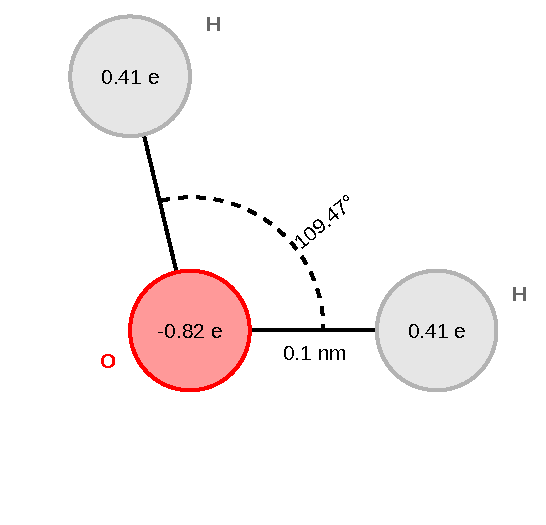
\includegraphics[scale=0.6]{H2O-SPCE-structure.pdf}
	\caption{Structure de la molécule d'eau selon le SPC (tiré de \cite{pullman_interaction_1981})}
	\label{fig:spc-structure}
\end{figure}

Ce modèle a été étendu avec le SPC/E pour prendre en compte la polarité de la molécule d'eau \cite{berendsen_missing_1987}.

	\subsection{ReaxFF}

ReaxFF \cite{russo_atomistic-scale_2011}\cite{senftle_reaxff_2016} est un potentiel utilisant les ordres de liaison pour modéliser des interactions atomiques en prenant en compte les réactions chimiques. Il a été conçu de façon à obtenir des résultats dont la précision se rapproche des méthodes quantiques, même en mettant en jeu autant d'atomes que les méthodes empiriques.\\
Cette méthode consiste à calculer les énergies atomiques et d'en déduire les forces (\autoref{fig:reaxff-interactions}).

\begin{figure}[hbpt]
	\centering
	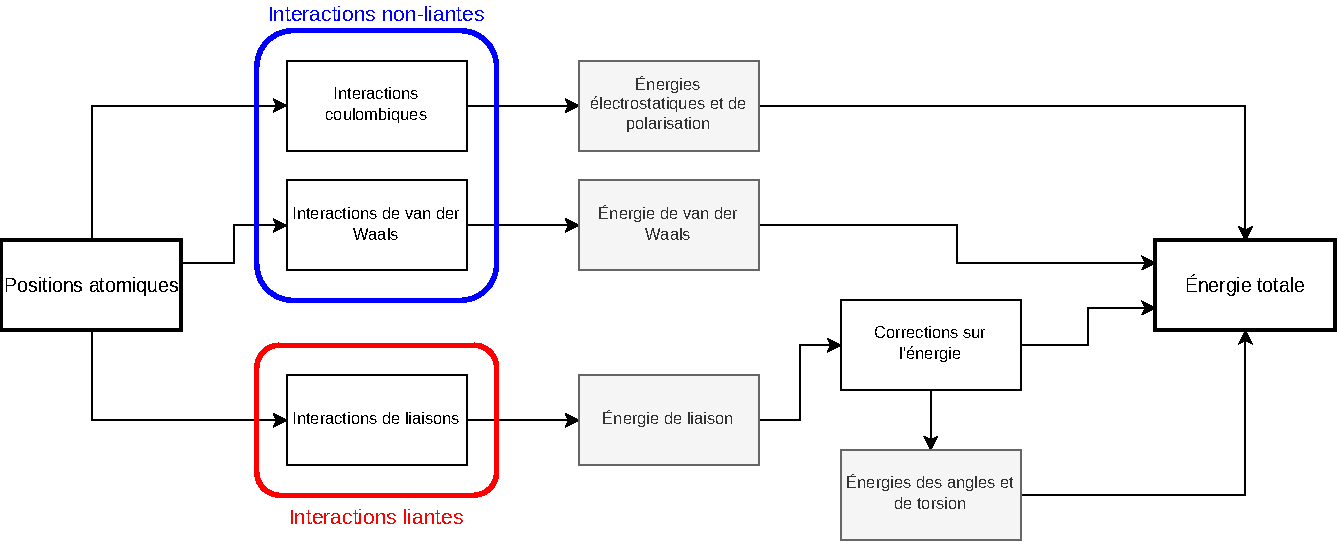
\includegraphics[width=\linewidth]{H2O-ReaxFF-interactions.pdf}
	\caption{Interactions et énergies au sein du ReaxFF (tiré de \cite{russo_atomistic-scale_2011})}
	\label{fig:reaxff-interactions}
\end{figure}

\section{Mise en place des simulations}

	\subsection{SPC/E}

Pour utiliser le modèle SPC/E dans LAMMPS, il faut fournir l'intégralité des liaisons, angles et molécules initiaux, paramétrer et utiliser le potentiel de Lennard-Jones ou hybride Lennard-Jones--Coulombien, et paramétrer les potentiels pour les liaisons et angles (\autoref{lst:parametrisation-spce}).

\begin{lstlisting}[caption={Exemple de paramétrisation pour utiliser le SPC/E}, label={lst:parametrisation-spce}]
...
pair_style    hybrid lj/charmm/coul/long 9.0 10.0
bond_style    hybrid harmonic
angle_style   hybrid harmonic
...
\end{lstlisting}

	\subsection{ReaxFF}

Pour utiliser ReaxFF dans LAMMPS, il faut fournir le fichier de configuration ReaxFF correspondant au système étudié, et utiliser le potentiel ReaxFF (\autoref{lst:utilisation-reaxff}).

\begin{lstlisting}[caption={Exemple d'utilisation du ReaxFF dans LAMMPS}, label={lst:utilisation-reaxff}]
...
pair_style   reax/c NULL
pair_coeff   * * test.reax O H
fix equilibration all qeq/reax 1 0.0 10 1e-06 reax/c
...
\end{lstlisting}

\section{Résultats obtenus}

Pour comparer ces systèmes, nous utilisons les grandeurs mesurées au cours des simulations, les fonctions de distribution radiale (\emph{Radial Distribution FUnction}, RDF) et les déplacements carrés moyens (\emph{Mean Squared Displacement}, MSD) obtenus.


\clearpage
\printbibliography

\end{document}